%\documentclass{article}
%\usepackage{graphicx}
%\begin{document}

\section{Population}
\label{Des:sec:population}
\begin{figure}[here]
\centering
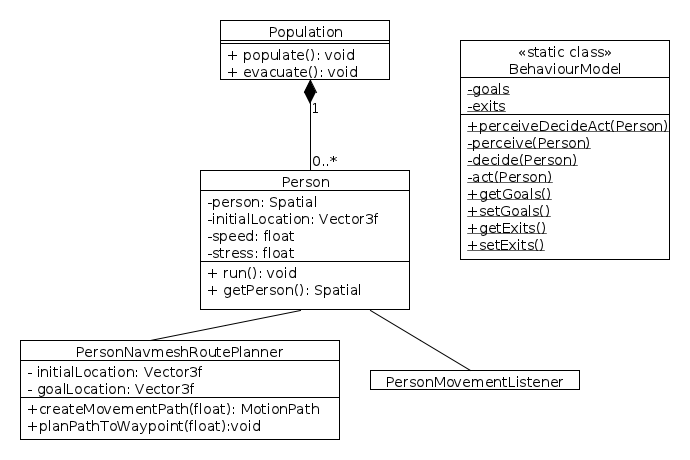
\includegraphics[scale = 0.5]{../UMLDiagrams/PopulationModel.png}
\caption{Population Package}
\label{fig:populationmodel}
\end{figure}


Figure \ref{fig:populationmodel} shows the relationship between the various classes responsible
for the realisation of autonomous agents and their behaviour within the simulator.
\\
The Population class represents the set of agents. A population instance is ran as a seperate thread of execution which
incrementally performs computations on the entire set of agents, such as computation of collision groups {REFERENCE collision/ORCA]. It is also responsible
for the generation of the set of agents using the information provided in a set of PersonCategories and the initiation
of agent evacuation.
\\
BehaviourModel is a static class designed to implement the Perceive, Decide, Act process [REFERENCE behavioural research]. For each step there is a corresponding 
private method which is called. The output from the perceive method, a list of goals visible to the agent, is passed to the decide method
which chooses a new target location for the agent to plan a path towards, and this location is passed to the act method which initiates the agents
movement towards its new goal.
\\
The seperation of these three stages is important to maximise the extensibility of the behavioural model. As mentioned, the decide method processes a set of
goals and, based on a set of rules and heuristics, chooses a new location for the agent. To change or extend the range of decisions an agent can make,
the programmer can simply add new rules to the decide method. In fact it is possible that multiple decision methods could be added where each implements
a different behavioural model [REFERENCE behavioural research]. The only restriction is that the decide method must take a set of Goals(see below) as one of its inputs and outputs 3D location.
By calling the perceiveDecideAct method, an agent is taken through all three stages of the process and need have no knowledge of the decision algorithms used to select this new goal.
\\

An agent is primarily realised by the three classes Person, PersonMovementListener and PersonNavmeshRoutePlanner. 
Each Person holds the attributes, including speed and stress [REFERENCE Behavioral Research] which represent the characteristics of 
an evacuee. It also coordinates the visual representation of an agent and the movement of the agent towards its goal.
\\
In order to plan a route to a location, a Person must create a PersonNavmeshRoutePlanner instance. It's purpose is to act 
as if it were a 'ghost' agent: it rapidly traverses the navmesh to establish a route. This route is then returned for the 
agent to move over. A fresh instance of PersonNavmeshRoutePlanner should be used every time a new route must be calculated and can be disposed
of once the route has been returned.
\section{Goals}
\label{Des:sec:goals}
\begin{figure}[here]
\centering
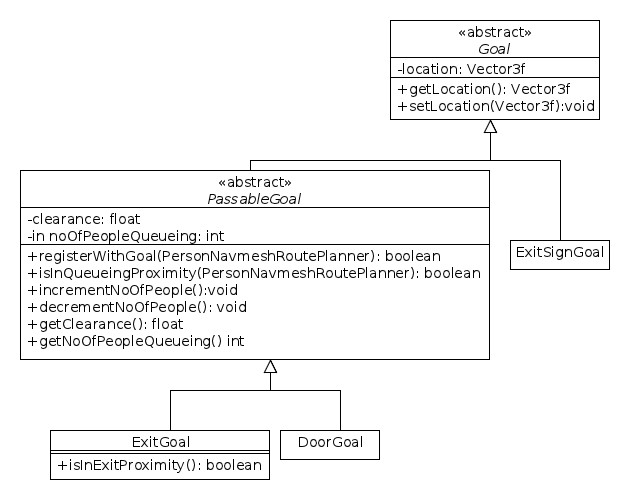
\includegraphics[scale=0.5]{../UMLDiagrams/GoalModel.png}
\caption{Hierarchy of goal package.}
\label{fig:goalhierarchy}
\end{figure}

A goal can be defined as anything in the environment which can steer an agents direction. Figure \ref{fig:goalhierarchy} shows the inheritance hierarchy for goals in this simulation. At the top level we define a generic Goal, which simply has a location and does not direct agents explicitly.
\\
A PassableGoal is any goal through which an agent can move, such as a door or exit. These also have a clearance; a radius around it's center which defines the maximum distance at which an agent can be considered to be queueing at that goal. This is vital for the computation of queueing behaviours. The number of people queueing at a PassableGoal is also stored and must be updated externally by agents as they approach or leave the goal.
Exits are represented by ExitGoals which are equipped with methods for recognising when an agent is close enough to exit the simulation.
\\
ExitSignGoal is an example of a non-passable goal which could direct agents to another goal. However non-passable goals are out of the scope of this project. ExitSignGoal is shown here purely to demonstrate that the existing framework could be extended to include such goals in future work.
\\
\\
\begin{figure}[here]
\centering
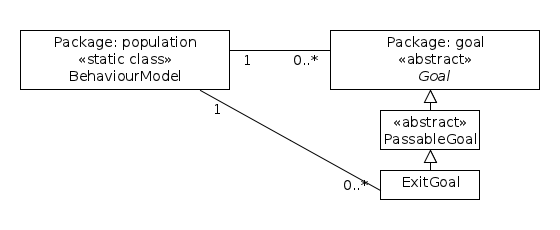
\includegraphics[scale=0.7]{../UMLDiagrams/BehaviourModelToGoalModel.png}
\caption{Relationship between BehaviourModel and Goals}
\label{fig:behaviourtogoalmodel}
\end{figure}

As figure \ref{fig:behaviourtogoalmodel} shows, the static BehaviourModel instance holds a collection of all Goals in the simulation. For the purposes of calculating agents paths out of the environment, a collection of all the ExitGoals is also kept seperately, since it is anticipated that these will be used most frequently in calculations.\\

%\end{document}

